%% It is just an empty TeX file.
%% Write your code here.

\section{Applications}

\begin{frame}
    \begin{center}
    \Huge Live Demonstration                
    \end{center}
\end{frame}

\begin{frame}[plain]
    \frametitle{Web GUI Demonstration}
    \begin{figure}
        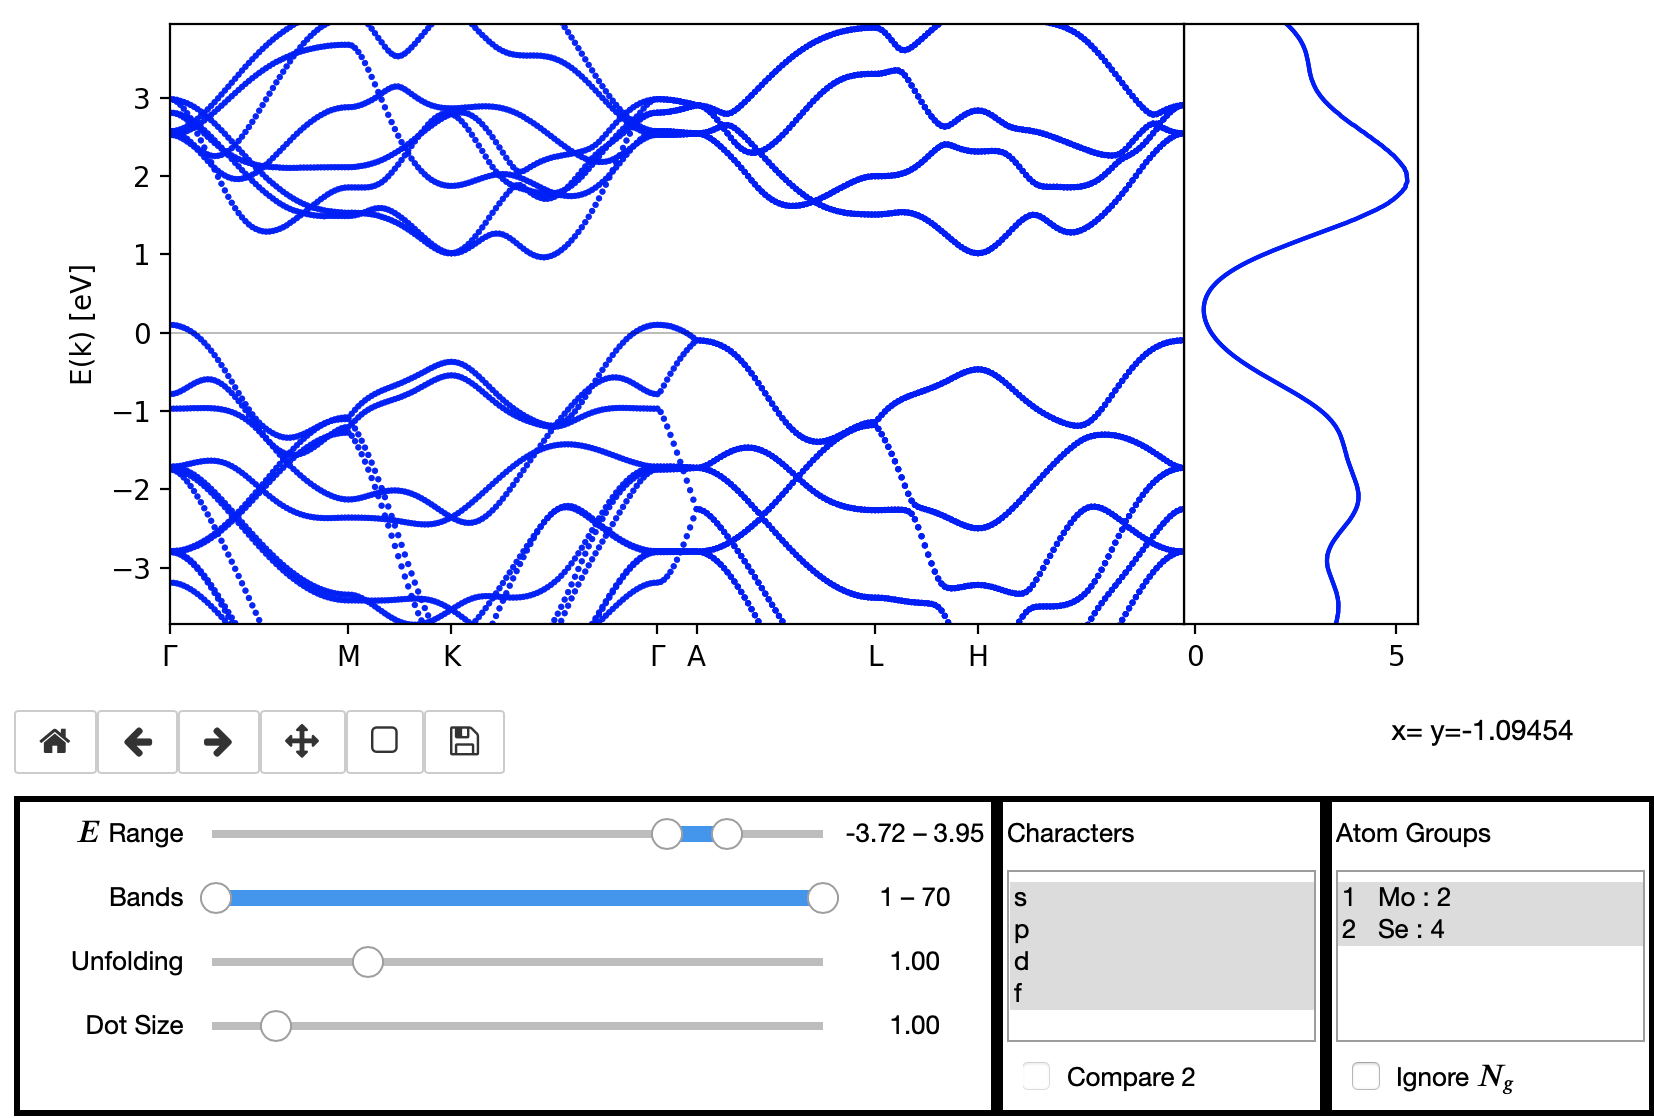
\includegraphics[width=1.0\textwidth]{data/screen1.png} 
    \end{figure}
\end{frame}

\begin{frame}[plain]
    \frametitle{Web GUI Demonstration}
    \begin{figure}
        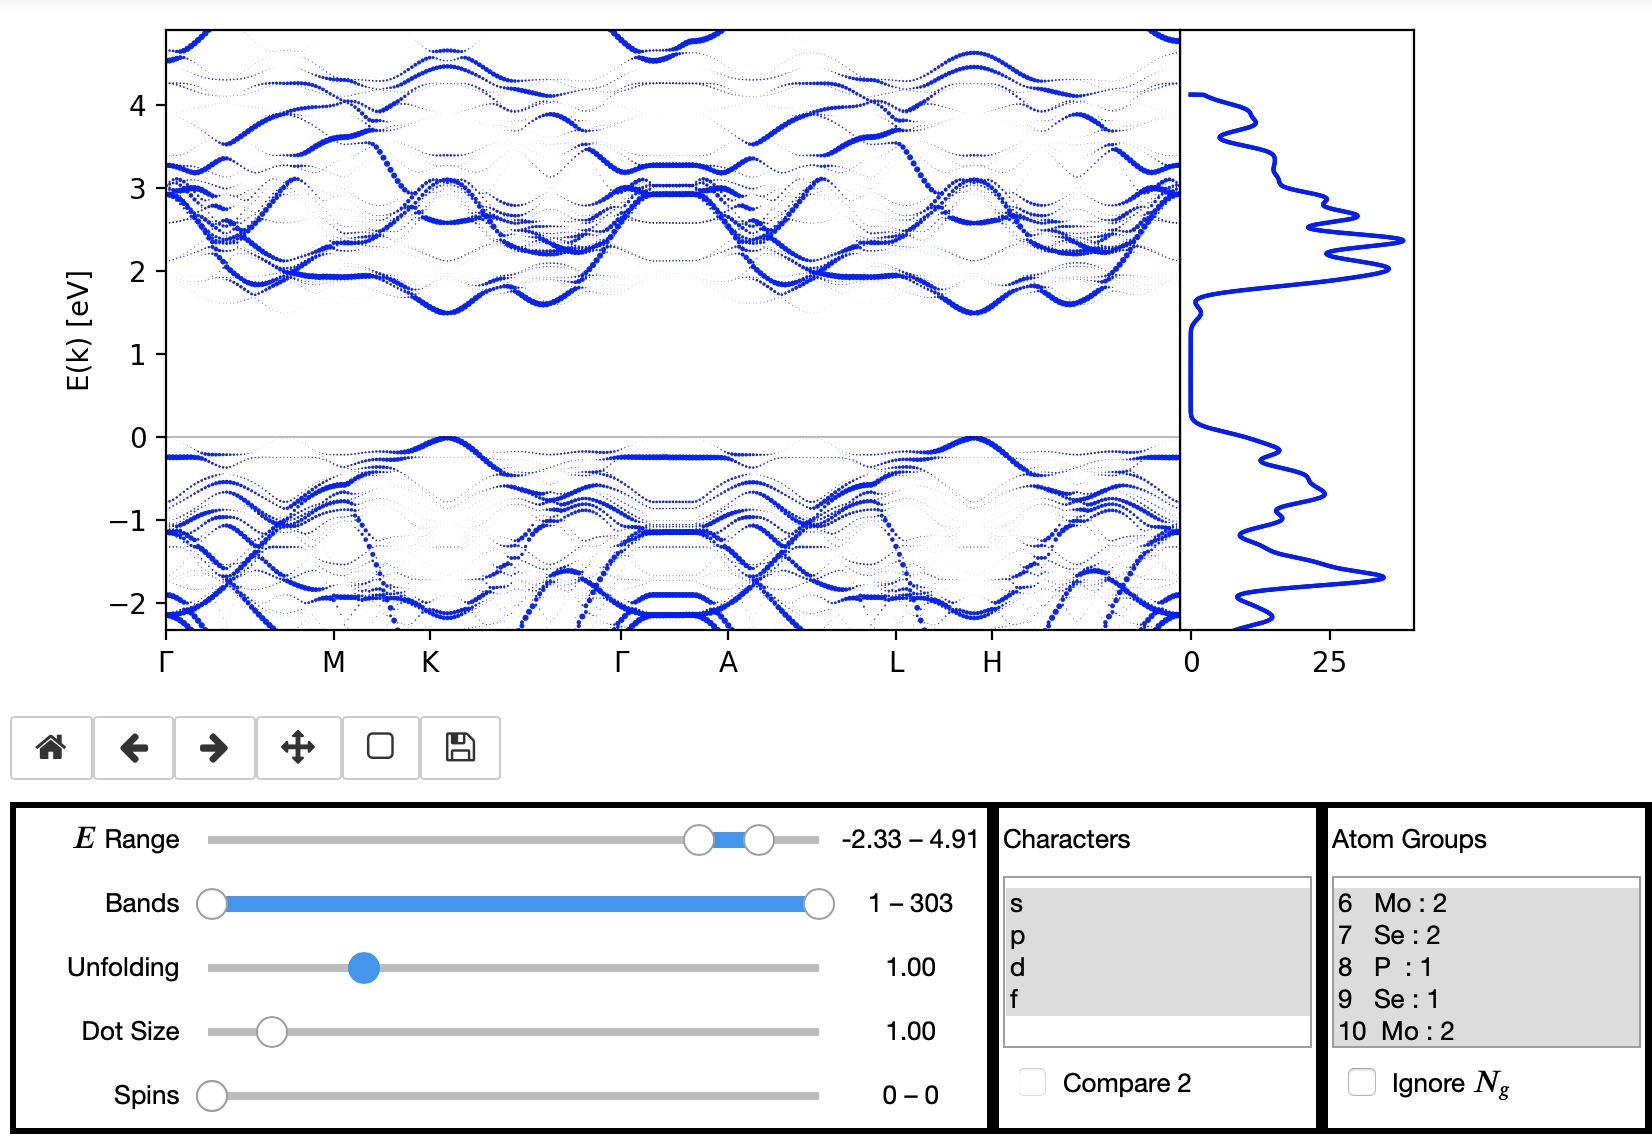
\includegraphics[width=1.0\textwidth]{data/screen2.png} 
    \end{figure}
\end{frame}

\begin{frame}[plain]
    \frametitle{Web GUI Demonstration}
    \begin{figure}
        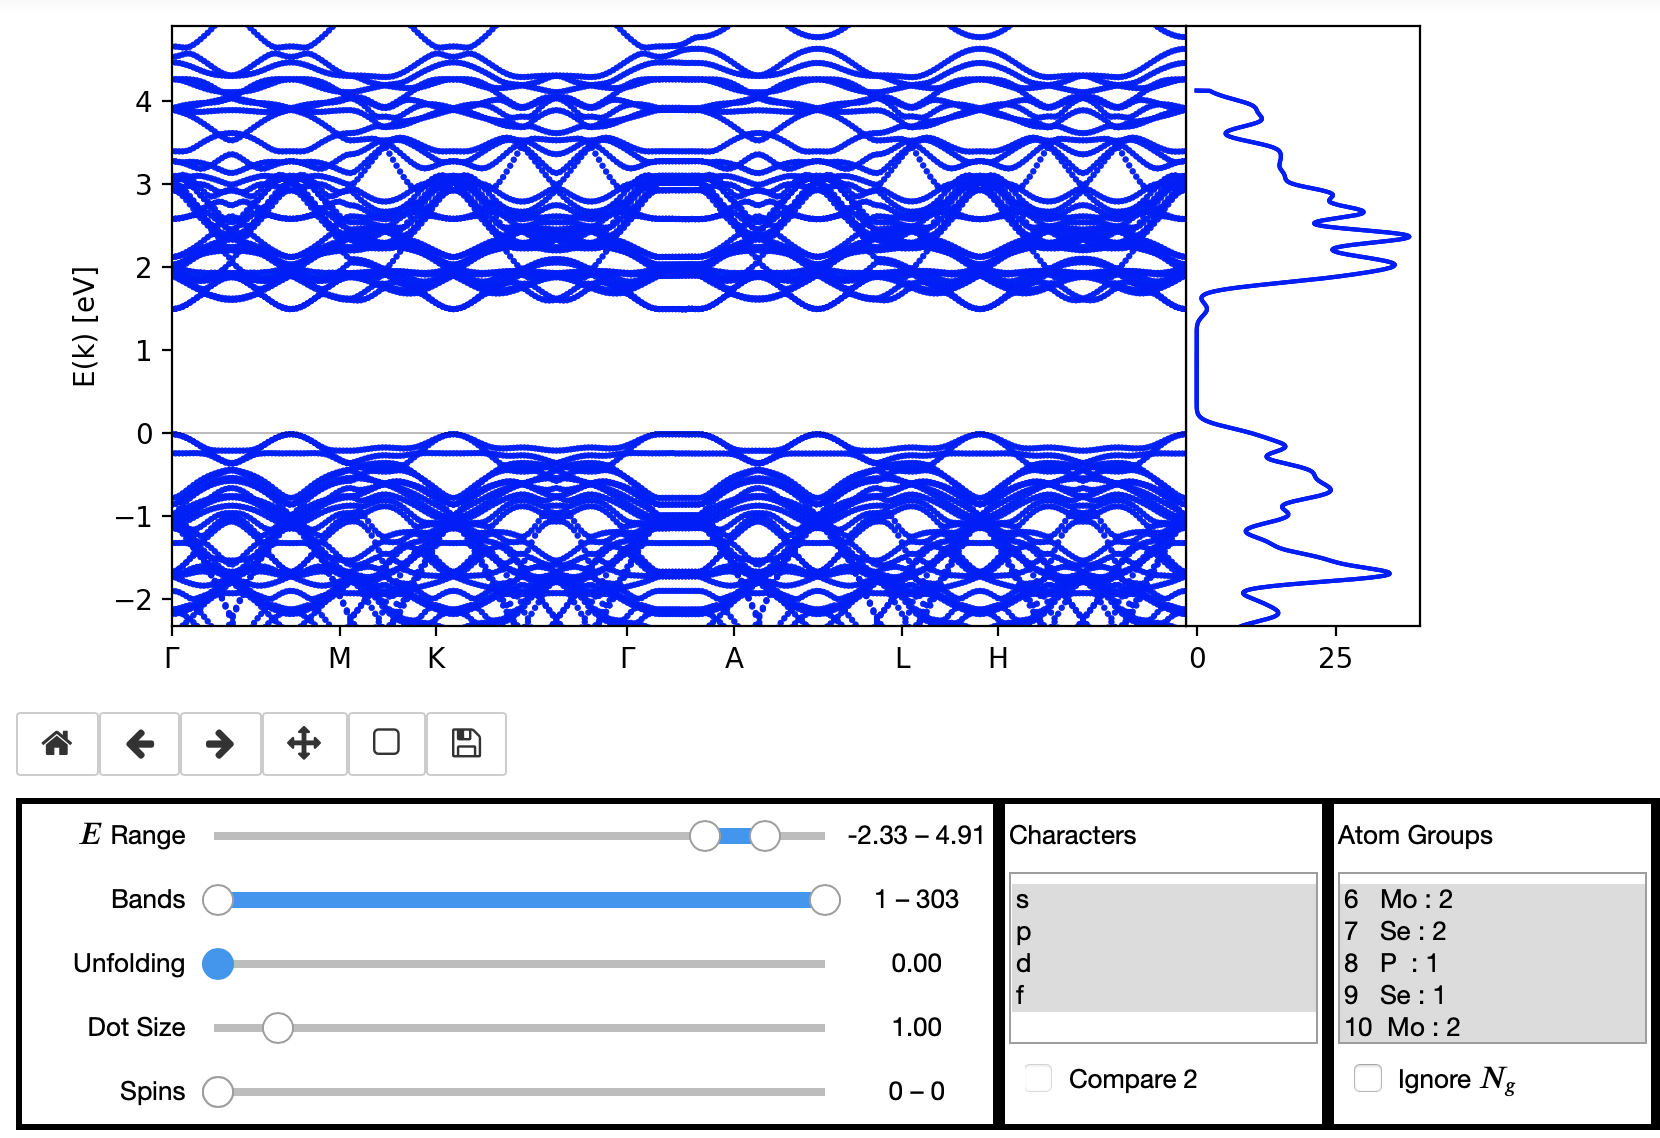
\includegraphics[width=1.0\textwidth]{data/screen3.png} 
    \end{figure}
\end{frame}

\begin{frame}\frametitle{Effective mass and group velocity:}
\begin{itemize}

\item Derived Quantities:

    \item Effective mass, that an electon in a crystal appears to have compared to a free electron (due to interactions in the solid)
    $m^{*} = \hbar^2  \left(\frac{\partial^2E(k)}{\partial k^2}\right)^{-1}$
    \
    \item Group velocity:
    $v_{G}(\vec{k}) = \frac{1}{\hbar}\frac{\partial E(\vec{k})}{\partial \vec{k}}$

    
    \item Problem: sparse k-Point mesh, but periodic bandstructure
    \item Idea: Using FFT to compute accurate derivates:
    \newline $\Leftrightarrow$ Differentiate a finite Fourier series
    \newline $f^{(n)}(x) = \mathcal{F}^{-1}\left((ik)^n\mathcal{F}(f(x))\right)$
\end{itemize}
\end{frame}

\begin{frame}
\begin{figure}
   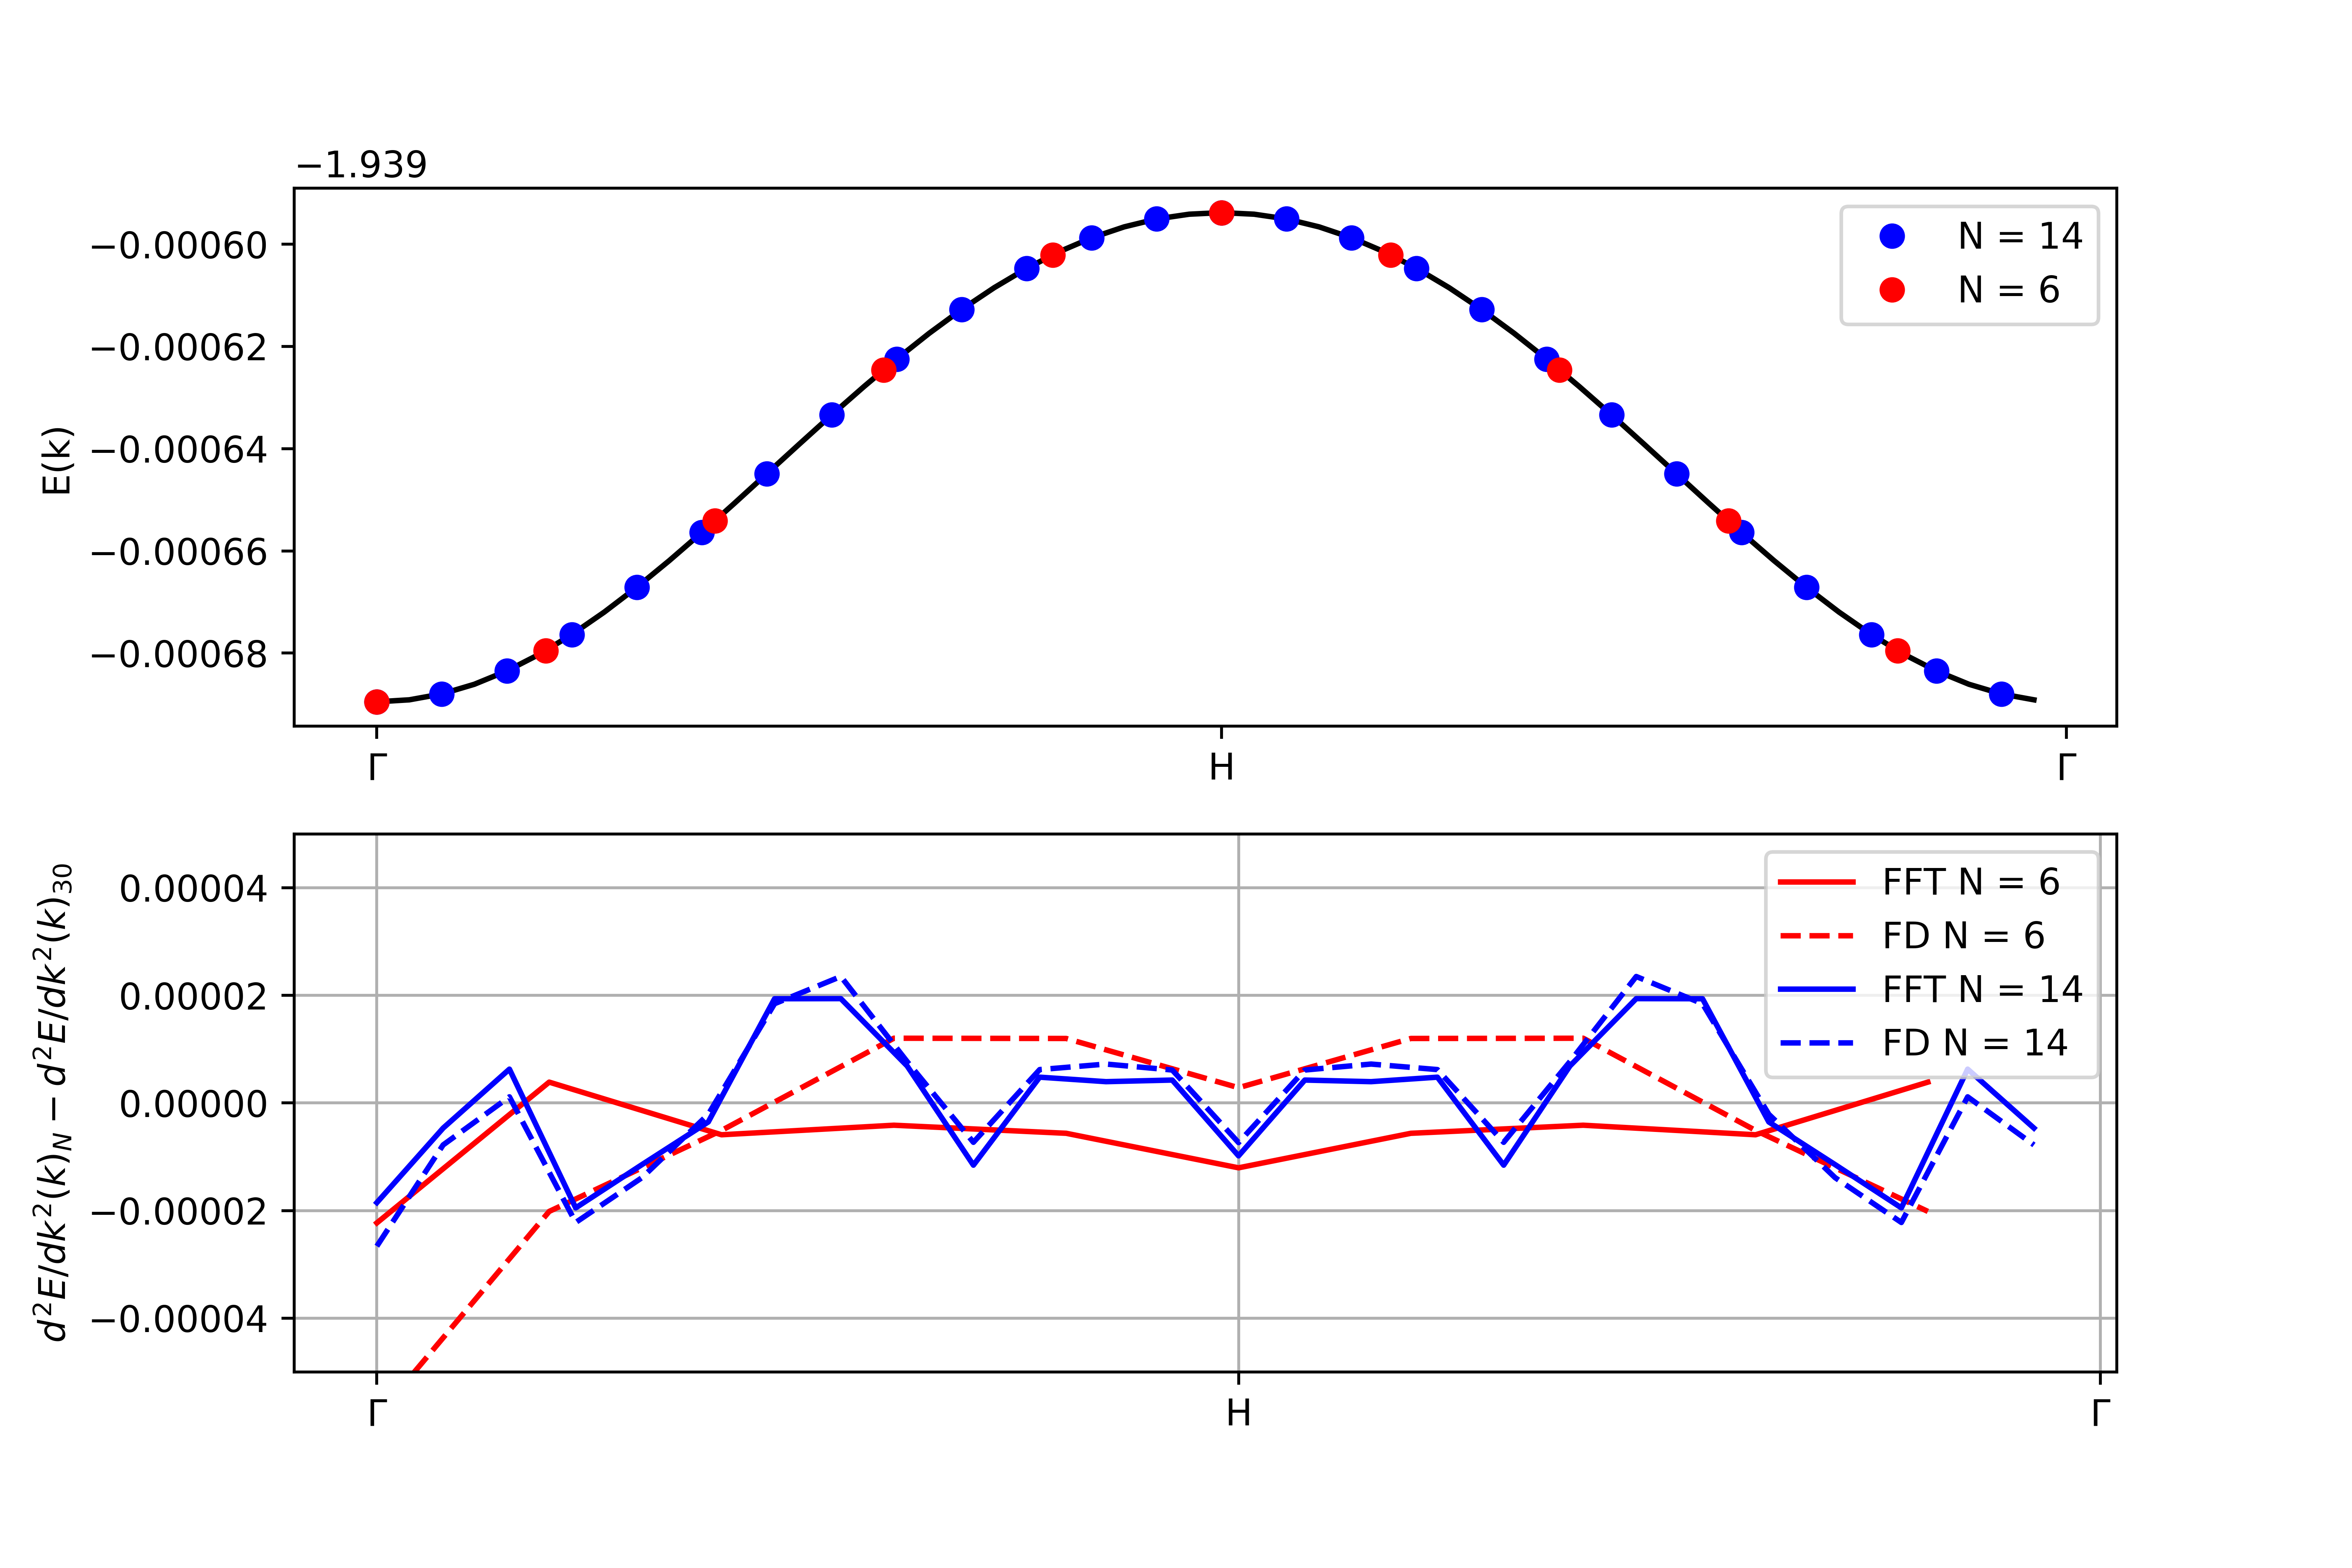
\includegraphics[width=1.0\linewidth]{data/diff_compare.png}
\end{figure}
\end{frame}



